\title{Computational Modelling in the Humanities and Social Sciences}
\author{mbkb74}
\date{}
\documentclass[11pt]{article}
\usepackage[a4paper, margin=2cm]{geometry}
\usepackage{graphicx}
\usepackage{float}
\usepackage[sorting=none]{biblatex}
\addbibresource{bibliography.bib}

\begin{document}
\maketitle

\section{Introduction}

The task I have chosen is to model the features of castles in England by geographic location. There are many ways in which a castle can be built, such as if it has a moat, a portcullis and so on.

\section{Sources of data and used modules}

The main source of data will be the National Heritage List for England by Historic England \cite{nhle}. Data will be obtained through this using Beautiful Soup, a web scraping tool for Python \cite{bs}. The data will then be processed by Stanza, a Natural Language Processing Python library \cite{qi2020stanza}. Data is then visualized using plotly in order to make the patterns clearer to see \cite{plotly}.

\section{Models and implementation}

The analysis of text uses multiple of the features from Stanza, first in using Part of Speech Tagging in order to find nouns and plural nouns in the sentences, as these are most likely to be the features I am looking for.

I am also using the provided lemmas feature in order to just extract the singular versions of the nouns, so that if in some cases a feature is discussed in plural, and in some cases singular, they will be treated the same. This has both benefits and drawbacks, providing a benefit in increasing the matching, however the use of the plural may convey information about the features, such as if a castle has multiple towers, compared to one tower.

The dependencies provided are also used to match together compound nouns, such as “Curtain wall”, as this provides more information than the separate nouns “curtain” and “wall”.

In order to categorize the castles into sections, I am using NUTS1 regions of England \cite{nuts}, this is an EU specification which divides up countries, in this case, dividing England into 9 regions. There is the option to get more granular with NUTS2 and NUTS3 regions being smaller than NUTS1, however given the limited dataset of around 230 castles, I wanted to ensure there were many castles per region so that the trends would be visible.

The location of each castle is extracted from the webpage, using an Ordnance Survey Grid Reference. This is then turned into latitude and longitude coordinates, which is finally converted into a NUTS region. One area in which this caused some trouble is in castles on small islands, as the converter must have been using a map that excluded these for performance. However the only case in which I discovered this was Lindisfarne castle, so not a significant proportion of the data, and so shouldn't affect the trends seen.

In order to simplify the categorization process, first I ran the code to generate an ordered list of features by how many times they occur. This list was then filtered to just the top 50 that I wanted to observe. This was done to ensure they were significant findings, as if it was just from one castle, it doesn't imply any trend. For these 50 features, a dictionary was created under each NUTS1 region with each features, and as the program went through the castles, the number was incremented if the feature was found in that region. Also kept track of was the total number of castles in each region so that the number of features could be divided by the number of castles to get an average value, ensuring that regions that just had more castles didn't look like they had more of a certain feature.


\section{Evaluation of models}

On evaluating the heatmaps, features did come out as showing as more prominent from certain areas, they can be shown below. You will see that London is white on this map as none of the castles in the dataset were in the London area.

The simplest evaluation of these results is to look at the description of building materials. Due to the difficulty of transportation at the time castles were being built, they use materials from the local area, and so they reflect geological surveys.

The most obvious of these are flint and sandstone, as shown below



\begin{minipage}{0.45\textwidth}
	\begin{figure}[H]
		\centering
		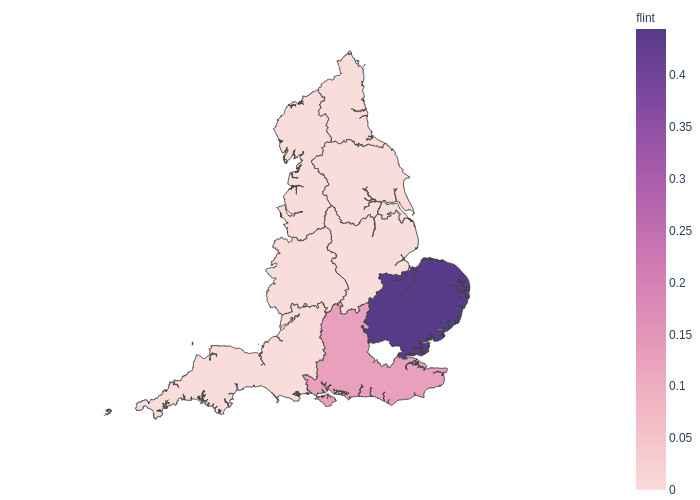
\includegraphics[width=\textwidth]{flint.png}
		\caption{Flint}
	\end{figure}
\end{minipage}
\begin{minipage}{0.45\textwidth}
	\begin{figure}[H]
		\centering
		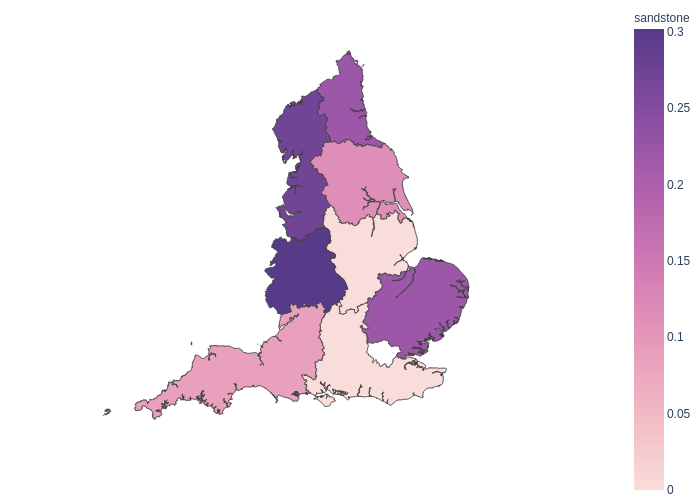
\includegraphics[width=\textwidth]{sandstone.png}
		\caption{Sandstone}
	\end{figure}
\end{minipage}
\vspace{1cm}
\\
Data from the British Geological Survey shows a large flint deposit in the south east area where flint is featured so heavily \cite{bgs}. Sandstone covers the west of England, curving round to the North East, with the rest featuring limestone instead. The image to view this needs to be seen at a large scale, and so it provided as an appendix at the end of this paper.

In addition to these two natural resources, the derivatives of natural resources can also be seen, with the South West using a lot more brick than other areas.

\begin{figure}[H]
	\centering
	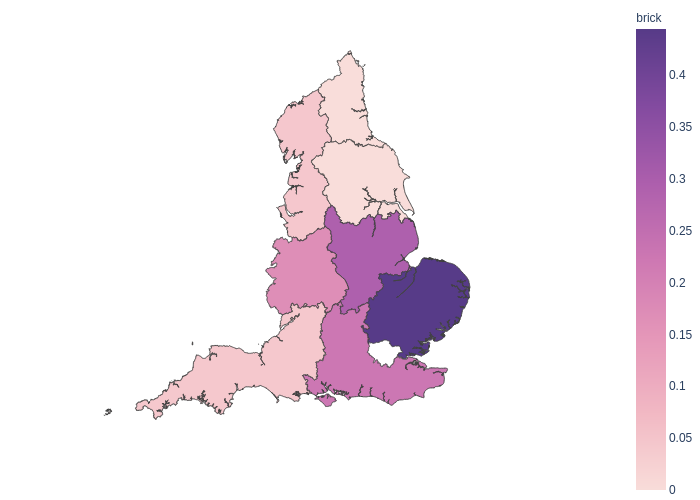
\includegraphics[width=0.45\textwidth]{brick.png}
	\caption{Brick}
\end{figure}

This is likely due to the large amount of Clay in the Thames valley, named the London Clay Formation \cite{sumbler1996london}.



% \begin{minipage}{0.45\textwidth}
% 	\begin{figure}[H]
% 		\centering
% 		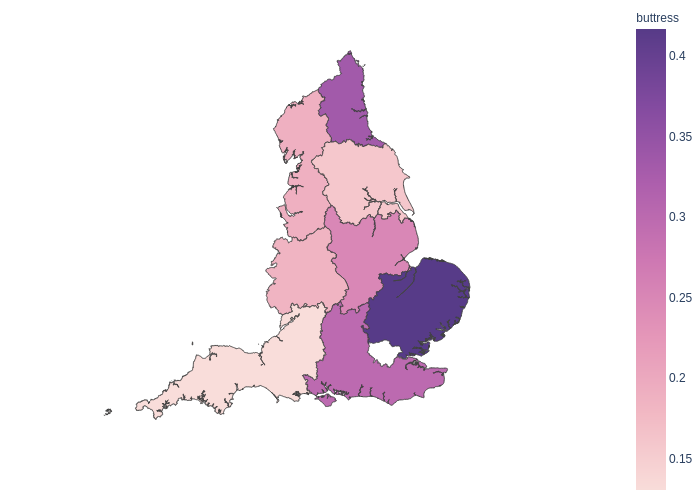
\includegraphics[width=\textwidth]{buttress.png}
% 		\caption{Buttress}
% 	\end{figure}
% \end{minipage}
% \begin{minipage}{0.45\textwidth}
% 	\begin{figure}[H]
% 		\centering
% 		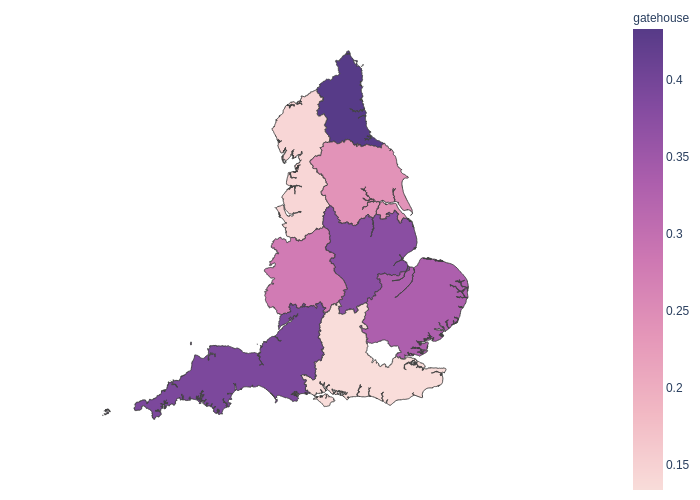
\includegraphics[width=\textwidth]{gatehouse.png}
% 		\caption{Gatehouse}
% 	\end{figure}
% \end{minipage}

% \begin{minipage}{0.45\textwidth}
% 	\begin{figure}[H]
% 		\centering
% 		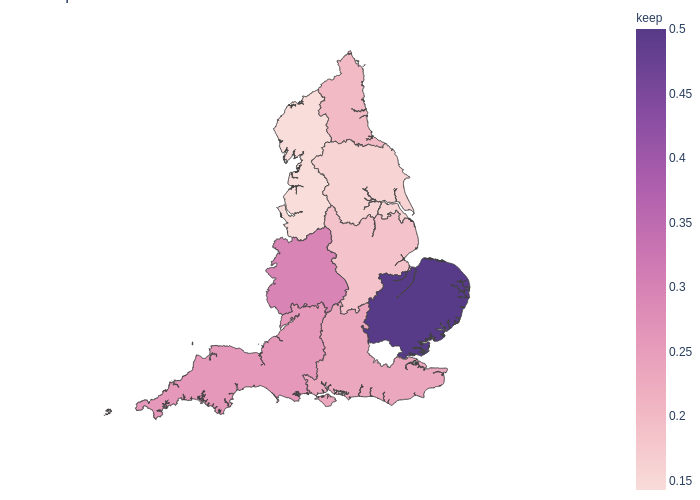
\includegraphics[width=\textwidth]{keep.png}
% 		\caption{Keep}
% 	\end{figure}
% \end{minipage}
% \begin{minipage}{0.45\textwidth}
% 	\begin{figure}[H]
% 		\centering
% 		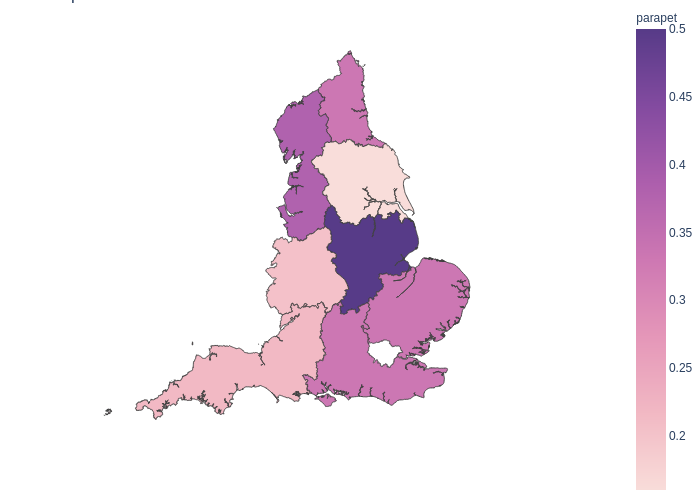
\includegraphics[width=\textwidth]{parapet.png}
% 		\caption{Parapet}
% 	\end{figure}
% \end{minipage}

% \begin{minipage}{0.45\textwidth}
% 	\begin{figure}[H]
% 		\centering
% 		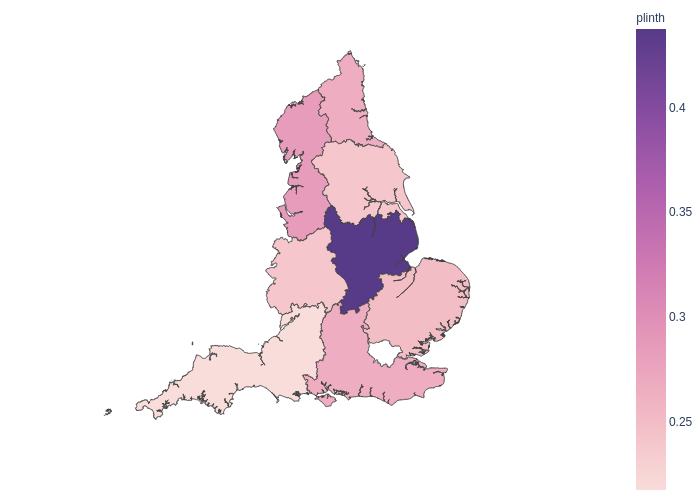
\includegraphics[width=\textwidth]{plinth.png}
% 		\caption{Plinth}
% 	\end{figure}
% \end{minipage}
% \begin{minipage}{0.45\textwidth}
% 	\begin{figure}[H]
% 		\centering
% 		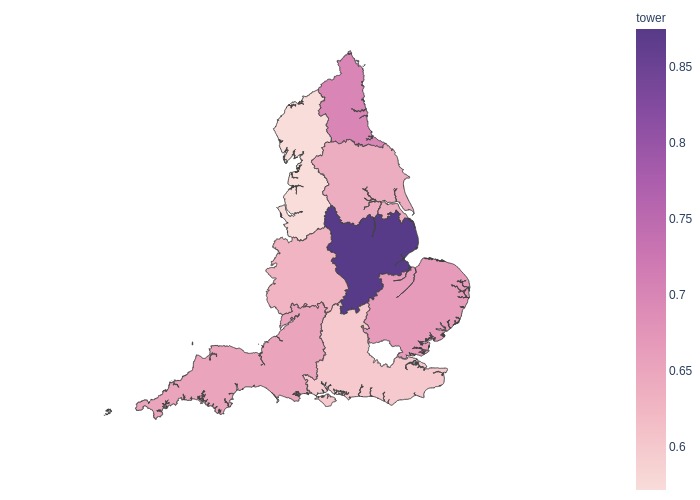
\includegraphics[width=\textwidth]{tower.png}
% 		\caption{Tower}
% 	\end{figure}
% \end{minipage}

% \begin{minipage}{0.45\textwidth}
% 	\begin{figure}[H]
% 		\centering
% 		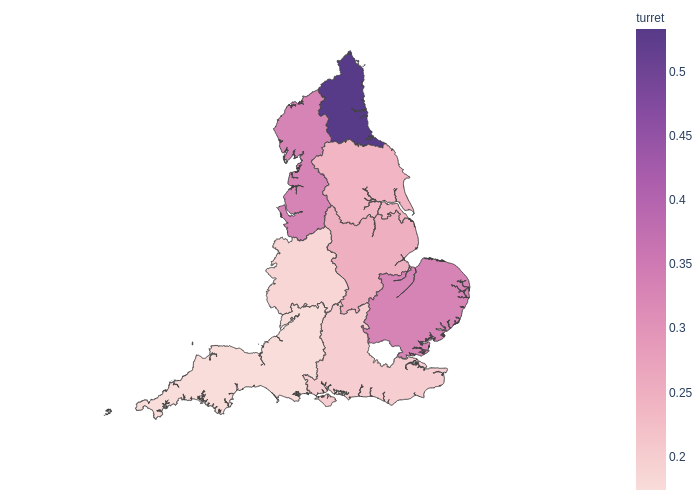
\includegraphics[width=\textwidth]{turret.png}
% 		\caption{Turret}
% 	\end{figure}
% \end{minipage}
% \begin{minipage}{0.45\textwidth}
% 	\begin{figure}[H]
% 		\centering
% 		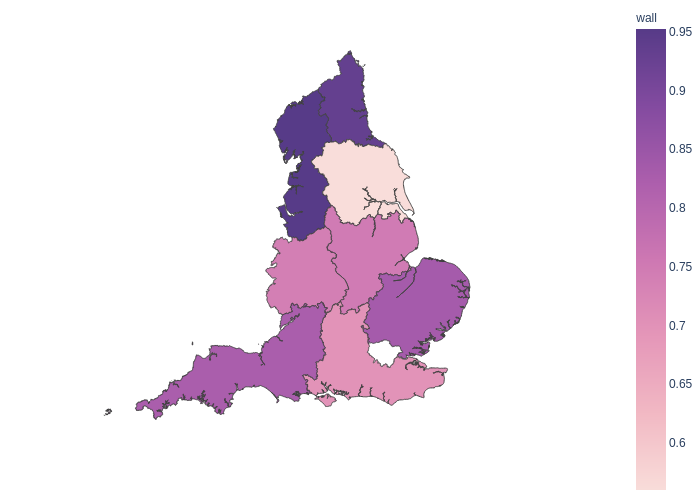
\includegraphics[width=\textwidth]{wall.png}
% 		\caption{Wall}
% 	\end{figure}
% \end{minipage}





\section{Conclusion}

\newpage
\printbibliography


\end{document}
